
\section{Technique}
\label{sec:approach}



We next describe our SQL query synthesis technique in detail.
How to infer the desirable query for the examples
shown in Section~\ref{sec:example} will
be discussed thoroughly in this section.

\begin{figure}[t]
  \centering
  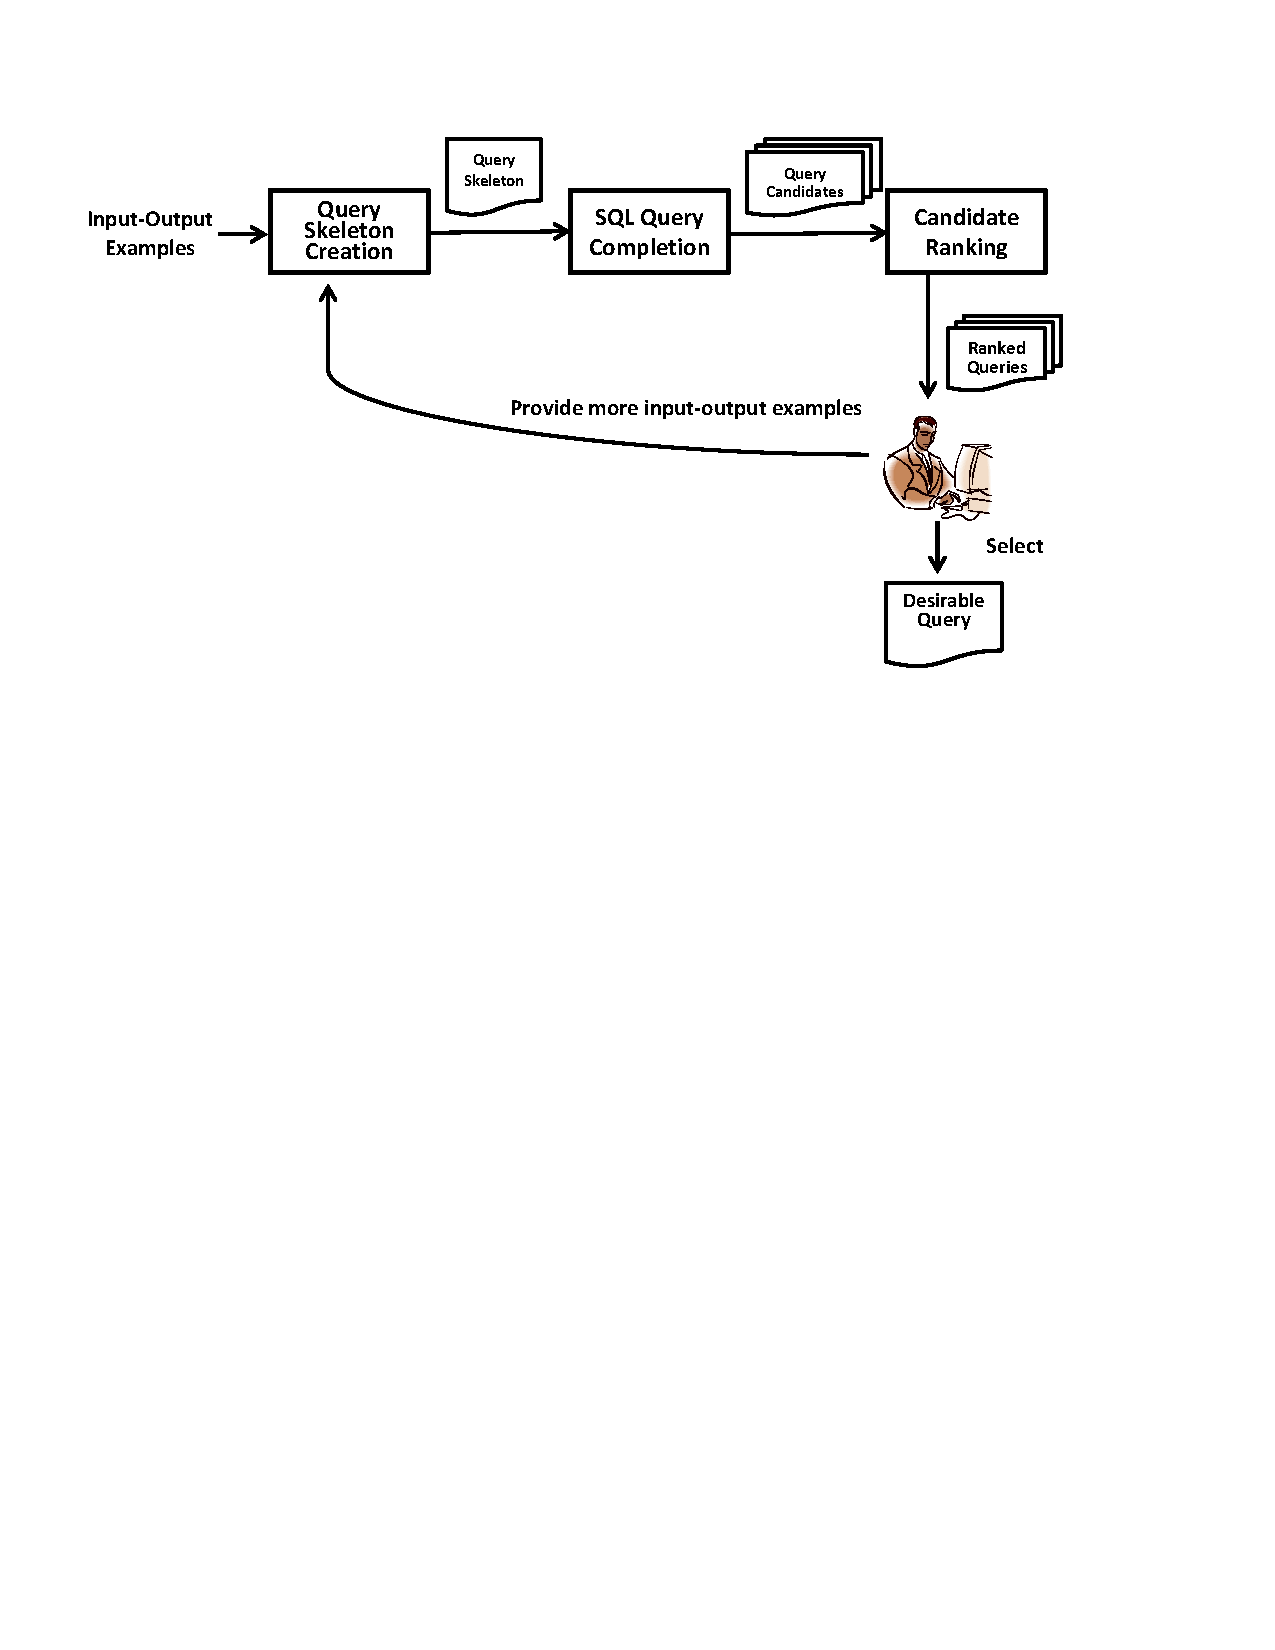
\includegraphics[scale=0.50]{workflow}
  \vspace*{-5.0ex}\caption {{\label{fig:workflow} The workflow of our SQL query synthesis approach.
}}

\end{figure}

\subsection{Overview}
Figure~\ref{fig:workflow} sketches the general workflow of our technique.
At a high level, our technique consists of three major steps: Query Skeleton
Creation(Section~\ref{sec:skeleton}), SQL Query Completion
(Section~\ref{sec:completion}), and Query Candidate Ranking (Section~\ref{sec:ranking}).
Specifically, our approach takes from users input-output examples. It first infers
a partially-complete query skeleton. The inferred query skeleton, though contains
incomplete parts that can not be yet decided, serves as a good reference
for further synthesizing a complete SQL query.
After that, our technique uses two techniques to complete a SQL skeleton.
In particular, it uses an advanced rule learning algorithm from the machine
learning community to infer query conditions (Section~\ref{sec:decision_tree}), and
 employs type-directed search to figure out possible aggregation
expressions (Section~\ref{sec:agg_search}).
The SQL Query Completion step produces a list of syntactically-valid
query candidates that satisfy the provided input-output examples.
However, it is possible that multiple query candidates can be synthesized based on the
provided input-output example. To deal with that, our technique
ranks all generated candidates,
and provides users a ranked list of SQL queries with the
simplest ones on the top. 
%This makes our tool more usable.


End-users can use our approach to obtain SQL query to transform
multiple, huge database tables by constructing small, representative
input and output example tables. On some examples, we speculate
that our approach
may produce a SQL query that satisfies the input and output examples
given by the user, but does not address the intention
that the user wants. To address this issue, we adapt a simple
interaction model from~\cite{Harris:2011} to ask users to investigate the results of
an output SQL query and report any discrepancy. In this case,
the user can refine the inferred SQL query by providing a more
informative input-output example (or multiple input-output examples
that together describe the required behavior) that demonstrate the behavior on
which the originally-inferred SQL query behaves incorrectly.

\subsection{Query Skeleton Creation}
\label{sec:skeleton}

In this step, our technique scans the provided input and output examples, guesses
what a target SQL query might look like, and infers a set of query skeletons
that capture the basic query structures.

A query skeleton is an incomplete SQL query, which
captures three basic query structures that could
often be decided after a simple scan over the examples:
tables used in a result SQL
query, table columns used to join input tables, and table
columns for projecting the query results. Other parts in a SQL query such as conditions
(including selection and having conditions), and aggregations
are left as unkown, and will be determinated in the next step (Section~\ref{sec:completion}).



%\begin{itemize}

%\item
\vspace{1mm}
\noindent \textit{\textbf{Step 1: Determining the Table Set.}} 
In practice, end-users are unwilling to provide more than enough
inputs. Therefore, every input table specified in the example
is expected to be used to construct a desirable SQL query.
Based on this observation, we assume that every input table
should be used as least once in the query. By default, the
table set $T$ used in the result SQL query contains all given input tables.
However, it is possible that a single table will be used for multiple times.
Our technique does not forbid this case, rather, we adopt a single heuristic
to estimate the used table set: if the same column from an input table appears more than once in the
example output, we add the input table the same number of times to the used table set.

%we view it as a strong indicator that this table will be joined multiple times and add it to our table
%set $T$ using an alias.


%\item
\vspace{1mm}
\noindent\textit{\textbf{Step 2: Determining Joining Columns. }} Given two arbitrary tables, there exist many
ways to join them. Enumerating all possible joining conditions may introduce a huge number of joining
conditions and would quickly become intractable. We observe that, in practice, two tables are often joined via the following
three cases: (1) tables are joined on their primary keys with the same (or compatible) data types, such
as joining a \textit{student} table with an \textit{enrolled} table with the \textit{student\_id} column. It does not
make any sense to join two tables on a Integer column and a String column; (2) tables are joined
using columns with the same name, such as joining a \textit{student} table with a \textit{enrolled} table on the
\textit{student\_name} column; and (3) two columns that have the data type, and have a large portion of
overlapped values in their corresponding input tables can be used as a joining condition. It is straightforward to check the first 
two cases to identify possible joining columns. For the third case, our technique scans the given input tables to check ``value similarity''
between two arbitrary columns, and selects columns whose ``value similarity'' is above a fixed threshold as joining columns.

%\item
\vspace{1mm}
\noindent \textit{\textbf{Step 3: Determining Output Columns.}} To identify output table columns on
which the querying result would be projected, our technique checks whether each output
table column name appears in any input tables. If so, we used the matched column
from the input table as the output column. Otherwise, the output column
must be produced by using aggregation. Our technique keeps track of those aggregation columns
and search for proper aggregates in the next phase (Section~\ref{sec:agg_search}). 

%After determining the table set and joining columns,
%the next step is to identify potential column names on which the result would be projected. If a
%column in the output table  does not appear in any input table's column list, this output column must
%be produced by aggregation. Our algorithm keeps track of these columns and appends a \CodeIn{group by} ... \CodeIn{having} ...
%clause to the query skeleton.

%\end{itemize}
\vspace{1mm}

In summary, this step infers three parts as a query skeleton: tables used in constructing a SQL query, joining conditions
to connect the input tables, and a list of columns to project the output results.

%It is worth noting that the results obtained from the above steps are not \textit{safe} in
%terms that they may miss some valid SQL queries. 

%We made the above assumption for the sake of tractability,
%since in theory, the bound of table number in a SQL query is $O(n_t!)$, where $n_t$ is the number of given tables;
%while the bound of possible number of join is $O(c_t^2)$ and the bound of the number of conditions is $O(n_t!n_tc_t^2)<O(n_t^3c_t^2)$.

%\subsubsection{Inferring Output Table Schema}

%Lacks schema

\subsubsection{Example}

For our motivating example, from the output table (Figure~\ref{tbl:output}), our technique identifies that
column {\CodeIn{Student\_name}} comes from table \CodeIn{student} and
column {\CodeIn{Max\_Score}} is a new one which must be created by using aggregation.
% which indicates aggregation and group by.

%while the bound of possible number of join is $O(c_t^2)$ and the bound of the number of conditions is $O(n_t!n_tc_t^2)<O(n_t^3c_t^2)$.

\begin{figure}[t]
	\centering
%\begin{CodeOut}
%\begin{alltt}
%\textbf{select student.Student\_name, $\color{blue}{<Aggregate>}$ 
%from student, enrolled
%where student.Student\_key = course.Student\_key
%      and \color{red}{<Conditions>}
%group by student.Student\_key
%having \color{red}{<Conditions>}}
%\end{alltt}
%\end{CodeOut}
%\vspace{-5mm}
		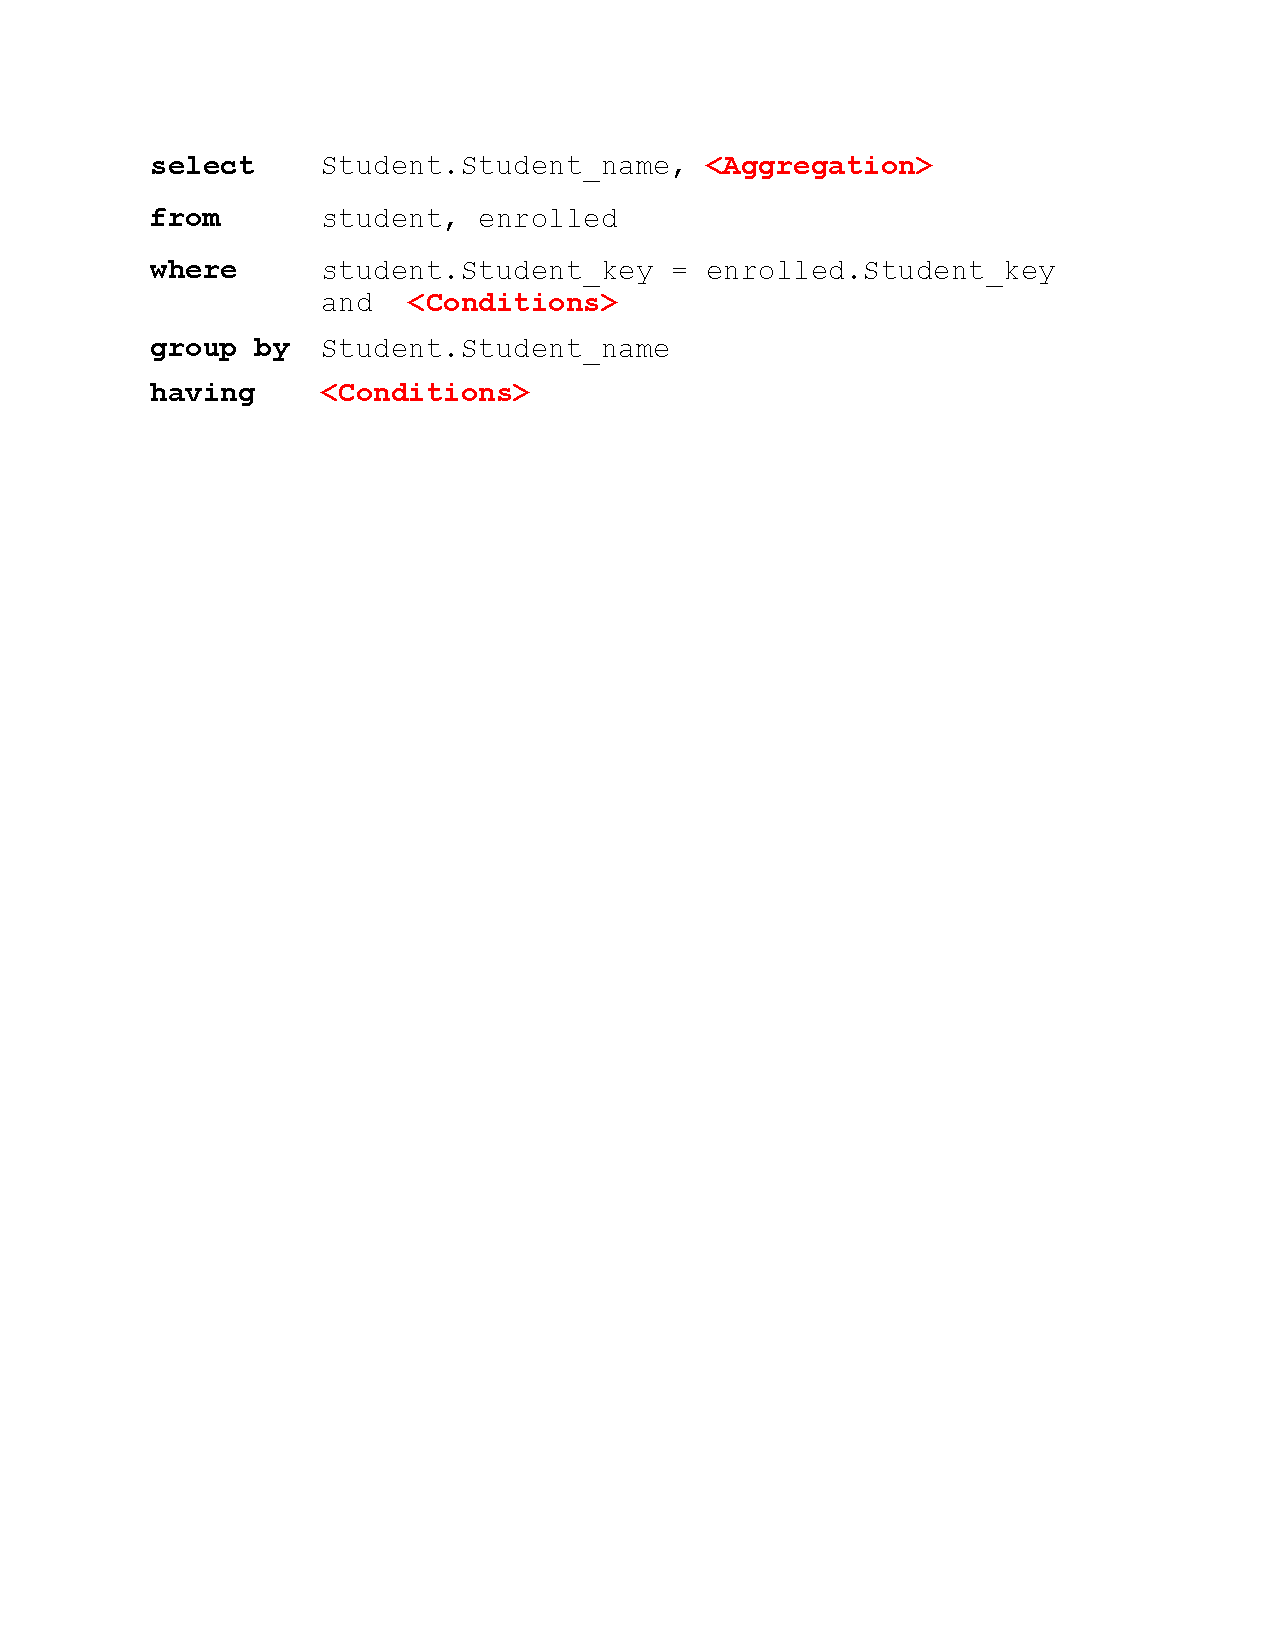
\includegraphics[width=0.45\textwidth]{sql_skeleton.pdf}
	\caption{The SQL skeleton created for the motivating example
in Section~\ref{sec:example}.}
	\label{fig:skeleton}
\end{figure}

The created query skeleton  is shown in Figure \ref{fig:skeleton}.
As we can see from Figure \ref{fig:skeleton},  there are three unknown structures represented
by $<$Aggregation$>$ or $<$Conditions$>$ in red color, which will be filled in the next phase.


\subsection{SQL Query Completion}
\label{sec:completion}

The SQL skeleton produced by the first step, though incomplete,
serves as a good reference in inferring complete and valid SQL queries.
In this step, our technique the remaining incomplete parts: conditions and
aggregates, by rule-based learning and type-directed search, respectively.

\subsubsection{Learning Conditions}
\label{sec:decision_tree}

The problem of learning query \textit{conditions} can be cast as finding
appropriate \textit{rules} that can perfectly divide the whole searching space
into positive part and negative part. In our context, the searching space
contains all tuples generated by joining the input tables, the positive part
are all tuples in the output table, and the negative part are the rest
tuples.

%the rest of tuples. Here our searching space consists of all tuples generated
%by joining input tables. These tuples can be returned by applying our SQL
%skeleton on input database if we remove all holes from the SQL skeleton.

Techniques to efficiently find rules from data has been studied extensively
by many machine learning researchers~\cite{Quinlan:1993, Cohen:1995, Frank:1998}.
Generally, in the machine learning community, there are major two paradigms of
rule learning:

%\begin{itemize}
%\item
\vspace{1mm}
\noindent\textbf{\textit{1. Decision-tree learning~\cite{Quinlan:1993}}}. Given
the positive and negative examples, one can generate a decision
tree, and then extract decision-tree-splitting conditions from the root to
all positive leaf. The extracted conditions can be viewed as the selection
criteria that isolates the output data from the input searching space.


%\item
\vspace{1mm}
\noindent\textbf{\textit{2.``Divide-and-conquer'' strategy~\cite{Pagallo:1990}}}. 
Unlike decision-tree learning, instead of learning a full tree,
this methodology repeatedly determines the most powerful rules for the dataset
that can maximally separate the positive examples from the negative ones, until
no more positive examples are available.

\vspace{1mm}

However, for our problem, both methodologies can not be directly applied.
Learning rules via decision-tree learning is restricted to conjunctive rules,
which is insufficient for many real scenarios. On the
other hand, the generalization ability of the ``divide-and-conquer'' strategy
is quite limited due to overpruning and covering heuristic.

To overcome these two limitations, in our technique, we adapt
the PART learning algorithm~\cite{Frank:1998}, which combines both
rule learning paradigms above. Notably, PART is capable of giving an more
accurate and expressive rule set. Specifically, it utilizes the
``divide-and-conquer'' strategy in that it repeatedly builds rules
and removes the instances it covers until no examples are left.
When creating each rule, it employs a pruned decision tree built from
current set of instance and only makes the leaf with the largest coverage
into the resulting rules, without keeping the whole learned tree in memory.


%In order to use PART, there are two issues that should be considered:

Although PART is a promising algorithm for learning rules from data,
there are two challenges when applying it to our problem:

%We customized PART in the following two aspects to make it applicable
%to our problem:

%\begin{itemize}
%\item
\vspace{1mm}
\noindent {\textbf{\textit{Challenge 1. How to represent tuples.}}}
%the literature of learning from examples~\cite{Mitchell:1997},
In PART, an example data point is represented by a single feature vector.
Therefore, we must transform tuples into appropriate feature representation.
To do so, a straightforward way is simply using concrete values in a tuple
as a feature vector. However, doing so loses much useful structure information
needed in a SQL query.

\vspace{1mm}
%\noindent {\textbf{\textit{Solution 1. Encoding prior knowledge.}}}
We encode existing domain knowledge about SQL query as additional
features, such as, (1) Aggregation, including \CodeIn{COUNT}, \CodeIn{MAX},
\CodeIn{MIN} and \CodeIn{AVG}, whose results might be used in query condition;
and (2) Comparison results between two comparable columns.
The above two additional knowledge encoding permits our technique
to make use of correlations between columns, rather than only values
from each isolated and sequential columns.

%Based on these observations
We add two types of new attributes into feature representation of tuples.

%indicate that not only columns themselves
%are useful for describing a tuple but we also should make use of correlation
%between columns. 

\begin{enumerate}

\item \textit{\textbf{Aggregation Features}}. Aggregation
features are the aggregation results grouped by each \CodeIn{String} type column
over every other columns. Table~\ref{tbl:agg} shows an example.


\item \textit{\textbf{Comparison Features}}. Comparison
feature is the result of comparing two comparable columns. We
consider two possible values:  $\{1, 0\}$,  which represents
means whether two columns under comparison satisfy the predicate or not, respectively.
Table~\ref{tbl:com} shows an example.

%the feature would be $0$. Suppose  the comparison features
%for them are summarized in Table \ref{tbl:com}.

\end{enumerate}

\begin{table}[t]
	\begin{center}
		\begin{tabular}{|c|c|}
		\hline
		\textbf{group by}	& \textbf{aggregation} \\
		\hline
		$C_1$ 				& \textsf{COUNT}($C_2$), \textsf{MAX}($C_3$), \textsf{MIN}($C_3$), \textsf{AVG}($C_3$)\\
		$C_2$ 				& \textsf{COUNT}($C_1$), \textsf{MAX}($C_3$), \textsf{MIN}($C_3$), \textsf{AVG}($C_3$)\\
		\hline
		\end{tabular}
	\end{center}
	\caption{The generated aggregation features for
a table with 3 columns:  $C_1$, $C_2$, and $C_3$, in which
columns $C_1$ and $C_2$ are \textsf{String} type and column $C_3$ is
\textsf{Integer} type.}
	\label{tbl:agg}
\end{table}



\begin{table}[t]
	\begin{center}
		\begin{tabular}{|c|c|}
		\hline
		\textbf{predicate}	& \textbf{comparison result} \\
		\hline
		$C_1=C_2$ 			& 0\\
		$C_1<C_2$ 			& 1\\
		$C_1>C_2$			& 0\\
		\hline
		$C_3=C_4$ 			& 1\\
		$C_3<C_4$ 			& 0\\
		$C_3>C_4$			& 0\\
		\hline
		\end{tabular}
	\end{center}
	\caption{The generated comparison features
for a table with 4 columns: $C_1$, $C_2$, $C_3$,
and $C_4$, in which columns $C_1$ and $C_2$ are \textsf{String} type, and
columns $C_3$ and $C_4$ are \textsf{Integer} type. Columns with
the same type are comparable, such as $C_1$ and $C_2$, and
$C_3$ and $C_4$.
}
	\label{tbl:com}
\end{table}

Combining using concrete tuple values, aggregation
features, and comparison features, our technique is able to
extract expressive feature representation for tuples,
and permits users to encode domain knowledge and structural
information about a SQL query.

%\item
\vspace{1mm}
\noindent {\textit{\textbf{Challenge 2. How to use the learnt rules to complete a SQL query.}}}
PART may return rules including three types of features. For example,
it returns the following rules for our motivating example in Section~\ref{sec:example}:
%. For our
%motivating example there is one rule learned from input tuples. It is

\smallskip
{
\CodeIn{COUNT(enrolled.Course\_key) $>$ 2}
    \CodeIn{\&\& student.level =`senior'}.
}
%\smallskip
\vspace{-2mm}

We need to split the returned rule into two parts: the query selection
condition, and the having condition. To achieve this, we
use $P_o$ to denote predicates related to original features
directly derived by the concrete tuple values,
$P_a$ to denote predicates related to aggregation features and $P_c$ to
denote predicates related to comparison features. For predicate in $P_o$,
we use it to fill condition holes in select clause by comparing selected
column with a constant value. For predicate in $P_a$, we
can use it to fill aggregation holes in having clause.

For our motivating example,
$P_o = \{\CodeIn{student.level =`senior'}\}$, 
$P_a = \{\CodeIn{COUNT(enrolled.Course\_key) $>$ 2}\}$.

After that, our technique adds a having condition such as ``\CodeIn{having COUNT(enrolled.Course\_key)}''
to the SQL query skeleton, and use predicates in $P_c$  to fill the selection condition.
%holes using predicates that compare two columns. There is no such predicate in our motivating example.

%\end{itemize}

\subsubsection{Searching for Aggregates}
\label{sec:agg_search}

The last step in completing a SQL query is searching for aggregates as the projection
columns. Our technique uses a type-directed searching strategy to do this. The whole
searching space includes all possible combinations of table columns and the five supported
aggregates (see Figure~\ref{fig:syntax}). In type-directed search, we leverage the following
information to prune the potential space:

\begin{enumerate}
\item The output values' type in the result column must be compatible with the aggregate's return
type. For instance, if an output column is String type, it must not use aggregates that always
return an Integer type, such as \CodeIn{count} and \CodeIn{sum}.

\item When using arithmetic aggregates such as \CodeIn{max} and \CodeIn{min}, the values
in the output column must have appeared in the input table.
\end{enumerate}

In our experience, the type-directed searching strategy significantly reduces the
searching space and makes our tool find the desirable aggregates faster.


\subsection{Query Candidate Ranking}
\label{sec:ranking}

After the above two steps, SQL queries satisfying the given input-output examples
will be returned. To reduce the effort in inspecting the
results and selecting a desirable query, we devise a strategy
to put the most likely query near the top of the return list.
%Due to lacking in input-output examples we are not be able to rule out SQL
%queries that lack in generalization ability. Instead we will provide user queries according to a rank.

Our strategy is based on Occam's razor to
compute a cost for each returned query, and prefers
queries with lower costs.
%queries in the increasing order of their costs.
For a SQL query, each table appearing in it introduces a cost $C_t$ and each appearing condition 
introduces an additional cost $C_p$. The total cost of a query is
computed by: $n_t \cdot C_t+n_p \cdot C_p$, where
$n_t$ is the number of tables and $n_p$ is the number of predicates used in the query. Our technique 
ranks queries based on their costs in an increasing order to ensure that a simpler query often ranks higher.
Figure~\ref{fig:rank} shows an example to illustrate this ranking strategy.


\begin{figure}[t]

\centering
\begin{tabular}{|l|l|}
%\hline
\multicolumn{2}{l}{Input table: \textbf{student}}\\\hline
%\hline
\textbf{name} & \textbf{score} \\\hline
Bob & 4  \\\hline
Dan & 5  \\\hline
Jim & 2  \\\hline
\end{tabular}
\quad
\begin{tabular}{|l|}
%\hline
\multicolumn{1}{l}{Query output}\\\hline
%\hline
\textbf{name}\\\hline
Bob  \\\hline
Dan  \\\hline
\end{tabular}

\vspace{2mm}


Query 1:
\vspace{-4mm}
\begin{CodeOut}
\begin{alltt}
\centering
\textbf{select name from student where score > 3;}
\end{alltt}
\end{CodeOut}

Query 2:
\vspace{-4mm}
\begin{CodeOut}
\begin{alltt}
\centering
\textbf{select name from student where name = `Bob` or name = `Dan`
}
\end{alltt}
\end{CodeOut}
\vspace{-5mm}
\Caption{{\label{fig:rank} The illustration of our query candidate ranking
strategy. Both Query 1 and Query 2 can transform the example input
to the example output. However, based on our ranking strategy, Query 1
is ranked higher, since it contains less conditions and is simpler
than Query 2.
An inferred query containing more conditions like Query 2 is more likely
to overfit the given examples.}}
\end{figure}



%\subsection{User Interactive Model}
%\label{sec:uim}


